\chapter{Massa dan Volume}\label{ch:g6:mass-and-volume}

Berapa banyak limun yang muat di dalam botol, dan seberapa \omterm{def:g4:weight-and-mass:weight}{berat} peti
berisi botol itu? Dua pertanyaan yang berbeda --- ruang dan zat ---
yang dengan riang dikusutkan menjadi satu kata oleh percakapan
sehari-hari, yaitu ``besar''. Sains menguraikannya: \omterm{def:g6:mass-and-volume:volume}{volume} untuk ruang
yang dipakai sebuah benda, \omterm{def:g3:measuring-mass:mass}{massa} untuk zat yang dikandungnya. Mengukur
yang kedua sudah kamu kuasai; hari ini kita belajar \omterm{def:g6:measurement-in-science:measuring}{mengukur} yang
pertama --- bahkan untuk kerikil yang bentuknya tidak mungkin disukai
penggaris mana pun.

\section{Volume: ruang yang dipakai sebuah benda}

\begin{definition}[Volume]\label{def:g6:mass-and-volume:volume}
Yang disebut \emph{volume}\index{volume} sebuah benda adalah banyaknya
ruang yang dipakainya. \omterm{def:g3:solids-liquids-gases:solid}{Zat padat}, \omterm{def:g3:solids-liquids-gases:liquid}{zat cair}, dan \omterm{def:g3:solids-liquids-gases:gas}{gas} semuanya punya
volume: batu bata memakai ruangnya, limun memakai bagian dalam
botolnya, \omterm{def:g2:air-around-us:air}{udara} memakai sisanya. Volume diukur dalam
\emph{sentimeter kubik}\index{sentimeter kubik} (\unit{cm^3}) --- yaitu
ruang sebuah kubus kecil yang tiap rusuknya satu \omterm{def:g2:measuring-length:units}{sentimeter} --- dan
dalam \emph{liter}\index{liter} (\unit{L}).
\end{definition}

\begin{proposition}[Liter dalam kubus]\label{prop:g6:mass-and-volume:litre}
Kedua keluarga \omterm{def:g6:measurement-in-science:measuring}{satuan} \omterm{def:g6:mass-and-volume:volume}{volume} itu sebenarnya satu keluarga:
\[
\qty{1}{L} = \qty{1000}{cm^3},
\qquad
\qty{1}{mL} = \qty{1}{cm^3}.
\]
Satu \omterm{def:g6:mass-and-volume:volume}{liter} tepat sama dengan ruang di dalam kubus yang tiap rusuknya
sepuluh \omterm{def:g2:measuring-length:units}{sentimeter}: $10 \times 10 \times 10 = 1000$ kubus kecil.
\end{proposition}

\begin{omfigure}
\begin{tikzpicture}[scale=0.85]
  \draw[thick] (0,0) rectangle (3,3);
  \draw[thick] (0,3) -- (0.9,3.75) -- (3.9,3.75) -- (3,3);
  \draw[thick] (3.9,3.75) -- (3.9,0.75) -- (3,0);
  \foreach \i in {1,...,9} {
    \draw[very thin] (0,0.3*\i) -- (3,0.3*\i);
    \draw[very thin] (0.3*\i,0) -- (0.3*\i,3);
    \draw[very thin] (0.3*\i,3) -- (0.3*\i+0.9,3.75);
    \draw[very thin] (3,0.3*\i) -- (3.9,0.3*\i+0.75);
    \draw[very thin] (0.09*\i,3+0.075*\i) -- (3+0.09*\i,3+0.075*\i);
    \draw[very thin] (3+0.09*\i,0.075*\i) -- (3+0.09*\i,3+0.075*\i);
  }
  \draw[thick, fill=omDef, fill opacity=0.6]
    (0,2.7) rectangle (0.3,3);
  \node[right, font=\small] at (4.6,3.0)
    {kubus besarnya: \qty{10}{cm} tiap rusuk};
  \node[right, font=\small] at (4.6,2.2)
    {$10 \times 10 \times 10 = 1000$ kubus kecil};
  \node[right, font=\small] at (4.6,1.4)
    {tiap kubus kecil: \qty{1}{cm^3}};
  \node[right, font=\small, omDef] at (4.6,0.6)
    {seluruhnya: $\qty{1000}{cm^3} = \qty{1}{L}$};
\end{tikzpicture}

{\small Satu \omterm{def:g6:mass-and-volume:volume}{liter}, dibongkar: seribu kubus sesentimeter yang ditumpuk
sepuluh kali sepuluh kali sepuluh.}
\end{omfigure}

\begin{example}[Volume yang perlu dihafal]\label{ex:g6:mass-and-volume:byheart}
Satu sendok teh memuat kira-kira \qty{5}{mL}; satu gelas minum
kira-kira \qty{25}{cL}, yaitu seperempat \omterm{def:g6:mass-and-volume:volume}{liter}; karton susu,
\qty{1}{L}; bak mandi, sekitar \qty{150}{L}; satu dadu gula memakai
kira-kira \qty{3}{cm^3}; satu dadu permainan kira-kira \qty{4}{cm^3}.
Jangkar seperti ini membuat langkah penilaian pada setiap pengukuran
menjadi mungkin.
\end{example}

\section{Mengukur zat cair}

\begin{method}[Membaca gelas ukur]\label{met:g6:mass-and-volume:cylinder}
Gelas takar milik laboratorium adalah \emph{gelas ukur}: tinggi,
sempit, berskala halus.
\begin{enumerate}
  \item letakkan gelas ukurnya di atas meja yang rata --- jangan
        pernah membacanya di tanganmu;
  \item carilah nilai satu undakannya, seperti pada setiap skala;
  \item sejajarkan matamu dengan permukaan \omterm{def:g3:solids-liquids-gases:liquid}{zat cairnya}: permukaannya
        tidak rata melainkan sedikit melengkung --- disebut
        \emph{meniskus}\index{meniskus} --- yang memanjat sedikit di
        dinding kacanya;
  \item bacalah pada \emph{dasar} lengkungannya, lurus mendatar.
\end{enumerate}
Mata terlalu tinggi atau terlalu rendah, dan lengkungannya berbohong
kepadamu sebesar satu dua undakan --- itulah kesalahan pandangan
menyerong dalam samaran kesayangannya.
\end{method}

\begin{omfigure}
\begin{tikzpicture}[scale=0.85]
  \draw[thick] (1.0,0) -- (1.0,4.2) (3.0,0) -- (3.0,4.2);
  \draw[thick] (1.0,0) -- (3.0,0);
  \fill[omDef, opacity=0.2] (1.0,0.05) rectangle (3.0,2.6);
  \draw[omDef, very thick]
    (1.0,2.75) .. controls (1.6,2.55) and (2.4,2.55) .. (3.0,2.75);
  \foreach \y/\l in {0.6/10, 1.4/20, 2.2/30, 3.0/40, 3.8/50} {
    \draw (3.0,\y) -- (3.25,\y);
    \node[right, font=\footnotesize] at (3.3,\y) {\l};
  }
  \draw[-Stealth, omThm, thick] (6.3,2.6) -- (2.2,2.6);
  \node[right, font=\small, omThm] at (6.4,2.6)
    {baca pada dasar lengkungannya: \qty{28}{mL}};
  \node[below, font=\small] at (2.0,-0.35)
    {mata sejajar permukaannya, gelas ukur di atas meja};
\end{tikzpicture}

{\small \omterm{met:g6:mass-and-volume:cylinder}{Meniskus}: \omterm{def:g3:solids-liquids-gases:liquid}{zat cair} memanjat sedikit di dinding kaca. Bacaan
yang jujur ada di dasar lengkungannya, dengan mata sejajar.}
\end{omfigure}

\begin{omfigure}
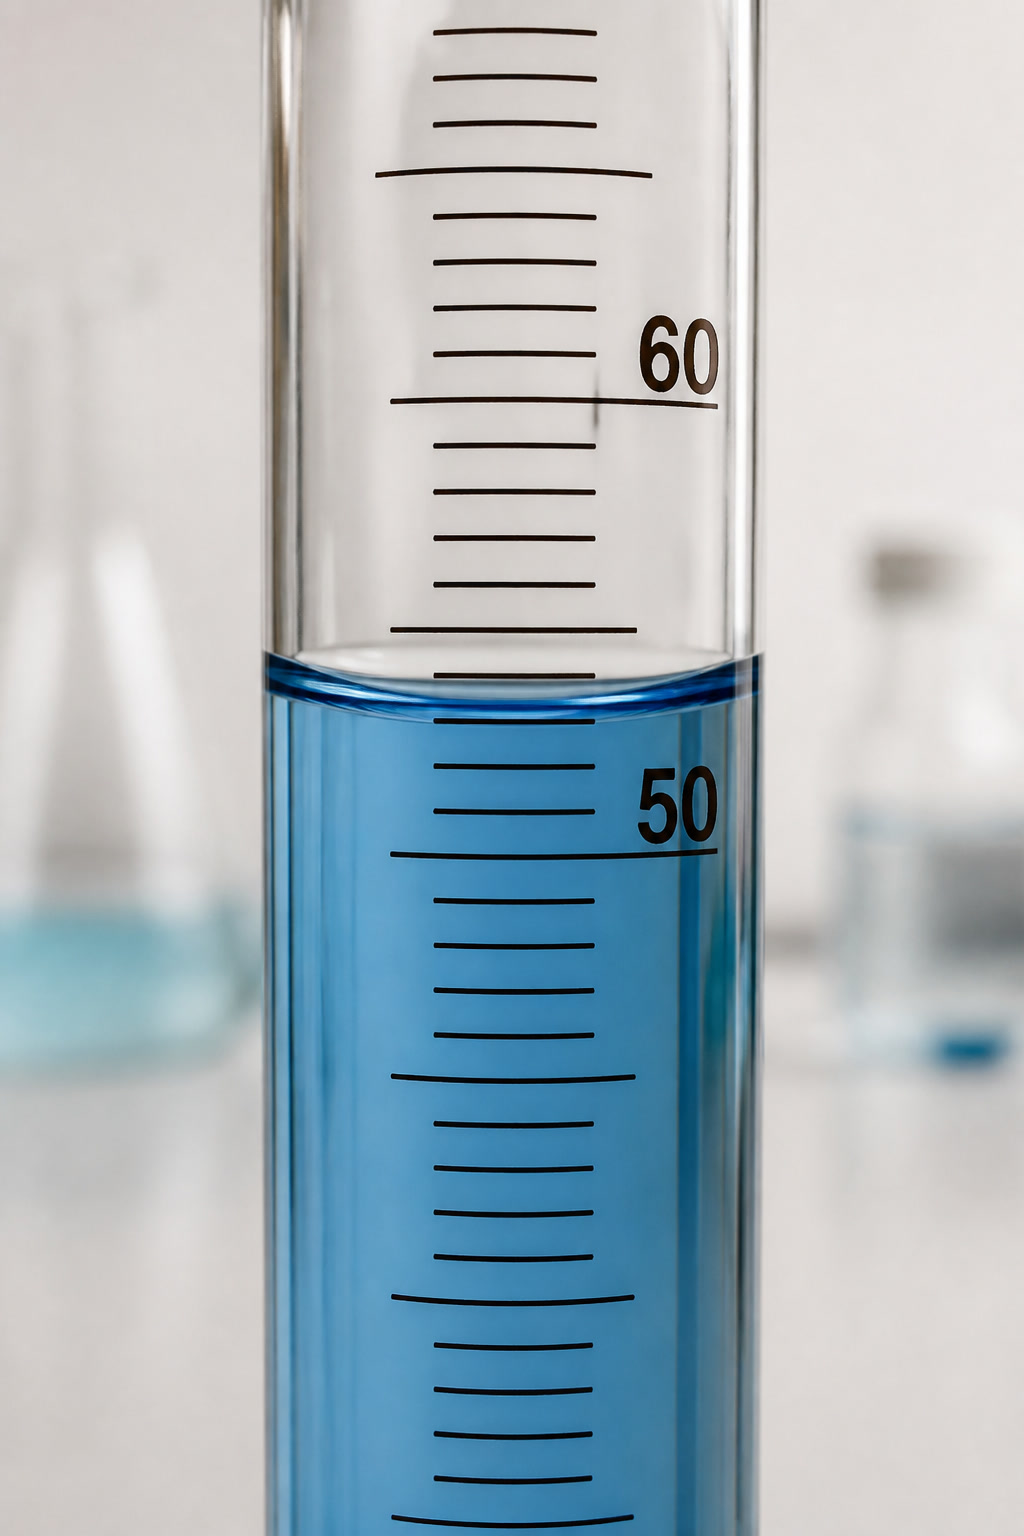
\includegraphics[width=0.3\linewidth]{images/book1/ai/g6-volume-cylinder.jpg}

{\small \omterm{met:g6:mass-and-volume:cylinder}{Meniskus} dari dekat: bacalah bagian tengahnya yang rata, dengan matamu sejajar dengannya.}
\end{omfigure}

\section{Mengukur zat padat --- bahkan yang bergumpal}

\omterm{def:g3:solids-liquids-gases:solid}{Zat padat} berbentuk balok menyerah kepada penggaris: panjang dikali
lebar dikali tinggi memberikan \omterm{def:g6:mass-and-volume:volume}{volumenya} dalam \unit{cm^3}, seperti
sudah ditunjukkan pelajaran matematikamu. Tetapi bagaimana dengan
kerikil, sebuah kunci, sebutir prem? Tidak ada penggaris yang cocok
untuk gumpalan. Jawabannya berumur dua ribu tahun, dan ia keluar dari
sebuah bak mandi.

\begin{proposition}[Pendesakan air]\label{prop:g6:mass-and-volume:displacement}
\omterm{def:g3:solids-liquids-gases:solid}{Zat padat} yang diturunkan seluruhnya ke dalam air mendesak air ke
samping --- tepat sebanyak \omterm{def:g6:mass-and-volume:volume}{volumenya} sendiri. Naiknya permukaan air
itu \omterm{def:g6:measurement-in-science:measuring}{mengukur} si penyusup: bergumpal atau licin, airnya membentuk
dirinya mengikuti setiap lekuk dan tonjolan.
\end{proposition}

\begin{method}[Volume dari naiknya air]\label{met:g6:mass-and-volume:rise}
\begin{enumerate}
  \item tuangkan air ke dalam gelas ukur --- cukup untuk
        menenggelamkan bendanya --- lalu bacalah \omterm{def:g6:mass-and-volume:volume}{volumenya}: misalkan
        \qty{120}{mL};
  \item ikatkan seutas benang pada bendanya lalu turunkan pelan-pelan
        sampai seluruhnya di dalam air, tanpa cipratan, tanpa
        menyentuh dindingnya;
  \item bacalah lagi: misalkan \qty{145}{mL};
  \item kurangkan: $145 - 120 = 25$ --- \omterm{def:g6:mass-and-volume:volume}{volume} bendanya
        \qty{25}{cm^3} (mililiter kenaikan, \omterm{def:g6:mass-and-volume:volume}{sentimeter kubik} batu:
        besaran yang sama).
\end{enumerate}
\end{method}

\begin{omfigure}
\begin{tikzpicture}[scale=0.85]
  \draw[thick] (0.8,0) -- (0.8,3.6) (2.6,0) -- (2.6,3.6)
    (0.8,0) -- (2.6,0);
  \fill[omDef, opacity=0.2] (0.8,0.05) rectangle (2.6,2.0);
  \draw[omDef, very thick] (0.8,2.0) -- (2.6,2.0);
  \node[right, font=\footnotesize] at (2.7,2.0) {120};
  \node[below, font=\small] at (1.7,-0.3) {sebelum};
  \draw[thick] (6.2,0) -- (6.2,3.6) (8.0,0) -- (8.0,3.6)
    (6.2,0) -- (8.0,0);
  \fill[omDef, opacity=0.2] (6.2,0.05) rectangle (8.0,2.42);
  \draw[omDef, very thick] (6.2,2.42) -- (8.0,2.42);
  \node[right, font=\footnotesize] at (8.1,2.42) {145};
  \draw (7.1,3.6) -- (7.1,1.0);
  \fill[omExo] (7.1,0.75) ellipse (0.4 and 0.3);
  \node[below, font=\small] at (7.1,-0.3)
    {sesudah: kerikilnya, seluruhnya di bawah air};
  \draw[-Stealth, omThm, thick] (4.0,2.0) -- (5.6,2.35);
  \node[below, font=\small, omThm] at (4.8,1.9)
    {kenaikan: \qty{25}{mL}};
\end{tikzpicture}

{\small Cara kenaikan air: airnya memanjat tepat sebanyak \omterm{def:g6:mass-and-volume:volume}{volume}
kerikilnya --- $145 - 120 = \qty{25}{cm^3}$ kerikil.}
\end{omfigure}

\begin{example}[Mahkota di dalam bak mandi]\label{ex:g6:mass-and-volume:archimedes}
Kisah lama: seorang raja mencurigai pandai emasnya mengencerkan emas
mahkota kerajaan dengan perak, lalu meminta ilmuwan Archimedes
mengetahuinya tanpa merusak mahkotanya. Ketika melangkah masuk ke bak
mandi yang penuh, Archimedes mengamati airnya tumpah melewati tepinya
--- dan seketika melihat bahwa limpahan itu \omterm{def:g6:measurement-in-science:measuring}{mengukur} \omterm{def:g6:mass-and-volume:volume}{volume} tubuhnya
sendiri, lengkap dengan segala gumpalannya. Konon ia berlari menyusuri
jalan sambil berteriak ``Eureka!'' --- \emph{aku sudah menemukannya!}
Bagaimana \omterm{def:g6:mass-and-volume:volume}{volume} mahkota itu membongkar kecurangannya memerlukan satu
gagasan lagi, dua bab di depan; bak mandinya memberi dia \omterm{def:g6:mass-and-volume:volume}{volume}
\emph{apa pun}.
\end{example}

\section{Massa dan volume adalah dua jawaban yang berbeda}

\begin{example}[Volume sama, massa berbeda]\label{ex:g6:mass-and-volume:different}
Isilah dua gelas \qty{25}{cL} yang serupa, satu dengan air, satu
dengan madu, lalu timbanglah keduanya (dengan mengurangi \omterm{def:g4:weight-and-mass:weight}{berat}
gelasnya): gelas berisi madu memuat jelas lebih banyak \omterm{def:g3:measuring-mass:units}{gram} di dalam
ruang yang persis sama. \omterm{def:g6:mass-and-volume:volume}{Volume} sama, \omterm{def:g3:measuring-mass:mass}{massa} berbeda. Dan satu \omterm{def:g6:mass-and-volume:volume}{liter}
\omterm{def:g2:air-around-us:air}{udara} \omterm{def:g4:weight-and-mass:weight}{beratnya} hampir tidak lebih dari satu \omterm{def:g3:measuring-mass:units}{gram}, di ruang tempat satu
\omterm{def:g6:mass-and-volume:volume}{liter} air \omterm{def:g4:weight-and-mass:weight}{beratnya} satu \omterm{def:g3:measuring-mass:units}{kilogram} penuh. Ruang dan zat memang dua juru
buku yang berbeda --- peganglah pikiran itu erat-erat: ia menjadi
sebuah hukum, dengan sebuah nama, pada bab terakhir tahun ini.
\end{example}

\begin{remark}[Menimbang yang tidak dapat berdiri sendiri]\label{rem:g6:mass-and-volume:tare}
Bagaimana menimbang tepung tanpa ikut menimbang mangkuknya? \omterm{def:g3:levers-and-scales:scale}{Neraca}
zaman sekarang punya tombol untuk itu: letakkan mangkuk kosongnya di
atas piring, tekan --- layarnya kembali ke nol --- lalu tuangkan:
\omterm{def:g3:levers-and-scales:scale}{neracanya} kini melaporkan tepungnya saja. Gerakan itu disebut
\emph{penaraan}. Tanpa tombolnya, timbanglah dua kali lalu kurangkan:
mangkuk-berisi-tepung dikurangi mangkuk kosong. Bagaimanapun caranya,
itu aturan permulaan yang adil lagi: mulailah dari nol yang jujur.
\end{remark}

\section{Latihan}

\begin{exercise}[$\star$]\label{exo:g6:mass-and-volume:1}
Pertanyaan apa yang dijawab \omterm{def:g6:mass-and-volume:volume}{volume}, dan pertanyaan apa yang dijawab
\omterm{def:g3:measuring-mass:mass}{massa}? Sebutkan dua \omterm{def:g6:measurement-in-science:measuring}{satuan} utama masing-masingnya.
\end{exercise}

\begin{exercise}[$\star$]\label{exo:g6:mass-and-volume:2}
Ubahlah: \qty{2}{L} menjadi \unit{cm^3}; \ \qty{350}{mL} menjadi
\unit{cm^3}; \ \qty{1500}{cm^3} menjadi \omterm{def:g6:mass-and-volume:volume}{liter}; \ setengah \omterm{def:g6:mass-and-volume:volume}{liter}
menjadi mililiter.
\end{exercise}

\begin{exercise}[$\star$]\label{exo:g6:mass-and-volume:3}
Mengapa gelas ukur harus dibaca dengan mata sejajar, di atas meja,
pada dasar meniskusnya? Sebutkan kesalahan yang dicegah tiap
aturannya.
\end{exercise}

\begin{exercise}[$\star$]\label{exo:g6:mass-and-volume:4}
Sebuah gelas ukur terbaca \qty{200}{mL}; dengan sebutir prem yang
diturunkan ke dalamnya, ia terbaca \qty{265}{mL}. Berapa \omterm{def:g6:mass-and-volume:volume}{volume}
premnya, dalam \unit{cm^3}?
\end{exercise}

\begin{exercise}[$\star$]\label{exo:g6:mass-and-volume:5}
Mengapa cara kenaikan air tetap bekerja untuk kerikil yang bergumpal,
padahal tidak ada penggaris yang dapat \omterm{def:g6:measurement-in-science:measuring}{mengukurnya}? Proposisi mana
yang menjawab?
\end{exercise}

\begin{exercise}[$\star$]\label{exo:g6:mass-and-volume:6}
Sebuah penghapus berbentuk balok berukuran \qty{5}{cm} kali
\qty{2}{cm} kali \qty{1}{cm}. Berapa \omterm{def:g6:mass-and-volume:volume}{volumenya}? Rencana pemeriksaan:
bagaimana kamu akan memastikannya dengan cara kenaikan air?
\end{exercise}

\begin{exercise}[$\star$]\label{exo:g6:mass-and-volume:7}
Untuk menimbang beras: mangkuk kosong \qty{280}{g}; mangkuk berisi
beras \qty{745}{g}. Berapa banyak berasnya? Tombol apa yang melakukan
pekerjaan yang sama dalam satu langkah?
\end{exercise}

\begin{exercise}[$\star$]\label{exo:g6:mass-and-volume:8}
Mana yang \omterm{def:g6:mass-and-volume:volume}{volumenya} lebih besar, sekilogram bulu atau sekilogram besi?
Mana yang \omterm{def:g3:measuring-mass:mass}{massanya} lebih besar? (Jawablah keduanya dengan cermat.)
\end{exercise}

\begin{exercise}[$\star\star$]\label{exo:g6:mass-and-volume:9}
Cara kenaikan air gagal untuk gabus: ia \omterm{def:g1:floating-and-sinking:words}{terapung}. Usulkan satu
perbaikan yang tetap memakai gelas ukurnya --- lalu katakan apa yang
harus dikurangkan kalau perbaikanmu memakai benda pembantu.
\end{exercise}

\begin{exercise}[$\star\star$]\label{exo:g6:mass-and-volume:10}
Sebuah karton jus mengaku berisi \qty{1}{L}. Ketika dituang, ia
mengisi gelas \qty{250}{mL} sebanyak tiga kali, dan gelas keempat
hanya sampai tanda \qty{200}{mL}. Jujurkah pengakuannya? Berapa
selisihnya?
\end{exercise}

\begin{exercise}[$\star\star$]\label{exo:g6:mass-and-volume:11}
Sebuah kalung diturunkan ke dalam gelas ukur yang terbaca
\qty{80.0}{mL}; permukaannya naik menjadi \qty{83.5}{mL}. Si pandai
emas mengaku kalung itu berisi \qty{5}{cm^3} emas. Mungkinkah
pengakuannya benar? Apa tepatnya yang diukur airnya?
\end{exercise}

\begin{exercise}[$\star\star\star$]\label{exo:g6:mass-and-volume:12}
Rancanglah pemeriksaan bergaya bak mandi terhadap
\cref{prop:g6:mass-and-volume:displacement} itu sendiri, dengan
memakai benda berbentuk balok yang \omterm{def:g6:mass-and-volume:volume}{volumenya} sudah diketahui
penggaris. Ceritakan langkahnya, ramalkan kedua bacaan gelas ukurnya
untuk balok berukuran $4 \times 3 \times 2$ \omterm{def:g2:measuring-length:units}{sentimeter} yang diturunkan
ke dalam \qty{150}{mL}, lalu nyatakan hasil apa yang akan membuktikan
proposisinya keliru.
\end{exercise}

\section{Soal: Hari Pembotolan di Kebun Buah}

\begin{problem}[{Soal akhir pekan --- hari pemerasan di kebun buah;
liter yang masuk botol, peti yang naik timbangan; kerikil di dalam
kendi}]\label{pb:g6:mass-and-volume:1}
Kebun buah itu memeras apelnya hari ini, dan setiap pembantu mendapat
satu pekerjaan \omterm{def:g6:measurement-in-science:measuring}{mengukur}.

\medskip\noindent\textbf{Bagian I --- Jus dalam \omterm{def:g6:mass-and-volume:volume}{liter}.}
Alat perasnya sudah mengisi satu tong \qty{20}{L}.
\begin{enumerate}
  \item Berapa \omterm{def:g6:mass-and-volume:volume}{sentimeter kubik} \qty{20}{L} itu?
  \item Jusnya dibotolkan dalam botol \qty{75}{cL}. Berapa botol
        \emph{penuh} yang dihasilkan tongnya?
  \item Berapa jus yang tersisa sesudah botol penuh yang terakhir,
        dalam sentiliter?
  \item Sisanya dituangkan ke dalam gelas \qty{25}{cL}. Berapa gelas
        yang terisi?
\end{enumerate}

\medskip\noindent\textbf{Bagian II --- Peti di atas timbangan.}
\begin{enumerate}[resume]
  \item Sebuah botol kosong bermassa \qty{450}{g}. Dengan memakai
        Bagian I, berapa \omterm{def:g3:measuring-mass:mass}{massa} jus di dalam satu botol penuh, kalau
        satu \omterm{def:g6:mass-and-volume:volume}{liter} jus bermassa kira-kira \qty{1}{kg}? (Kerjakan
        dalam \omterm{def:g3:measuring-mass:units}{gram}.)
  \item Jadi berapa \omterm{def:g4:weight-and-mass:weight}{berat} satu botol penuh seluruhnya?
  \item Sebuah peti kayu \omterm{def:g4:weight-and-mass:weight}{beratnya} \qty{2}{kg} dalam keadaan kosong
        dan memuat enam botol penuh. Berapa \omterm{def:g3:measuring-mass:mass}{massa} total satu peti
        yang bermuatan?
  \item Mobil boks itu boleh membawa \qty{200}{kg} peti. Berapa peti
        bermuatan yang boleh diangkutnya? (Hanya peti yang utuh.)
\end{enumerate}

\medskip\noindent\textbf{Bagian III --- Kerikil di dalam kendi.}
Tom kecil menjatuhkan sebutir kerikil ke dalam kendi jus \qty{1}{L}
yang penuh, dan jusnya melimpah ke atas meja.
\begin{enumerate}[resume]
  \item Limpahan yang dilap itu terukur \qty{40}{mL}. Apa yang
        diukur tumpahan itu tentang kerikilnya, dan menurut
        proposisi yang mana?
  \item Sesudah kerikilnya diambil, berapa jus yang tersisa di dalam
        kendinya?
  \item Tom membantah: ``Kerikilnya kecil --- lihat, ia sembunyi di
        dalam kepalan tanganku!'' Kakaknya menjawab dengan gelas
        ukur: ia memasukkan kerikilnya ke dalam \qty{100}{mL} air.
        Bacaan berapa yang membuktikan tumpahannya berkata benar?
  \item Pembukuan tambahan: kerikilnya \omterm{def:g4:weight-and-mass:weight}{beratnya} \qty{104}{g} pada
        timbangan dapur. Tanpa gagasan baru apa pun, sudah dapatkah
        kamu mengatakan apakah zat kerikil lebih berat atau lebih
        ringan daripada zat jus \emph{untuk ruang yang sama}?
        Bandingkan \qty{104}{g} kerikil dalam \qty{40}{cm^3} dengan
        \omterm{def:g3:measuring-mass:mass}{massa} jus yang akan mengisi \qty{40}{cm^3} yang sama itu ---
        lalu simpanlah kesimpulanmu tetap hangat untuk bab \omterm{def:g3:measuring-mass:mass}{massa}
        jenis.
\end{enumerate}
\end{problem}
